% Set the author and title of the compiled pdf
\hypersetup{
	pdftitle = {\Title},
	pdfauthor = {\Author}
}

\section{Distributed computing}
% Lecture One

A distributed system is a computing platform build with many computers that:

\begin{itemize}
  \item Operate concurrently,
  \item Are physically distributed (and can fail independently)
  \item Are linked by a network
  \item Have independent clocks
\end{itemize}

Leslie Lamport once said that:

\begin{aquote}{Leslie Lamport}
You know you have a distributed system when the crash of a computer you’ve never
heard of stops you from getting any work done.
\end{aquote}

The consequences of having a distributed system is that many problems can arise
from a lack of synchronization and coordination between parts of the system.
Problems include:

\begin{itemize}
  \item Non-determinism
  \item Race conditions
  \item Deadlocks and synchronization
  \item No notion of a correct time (no global clock)
  \item No (visible) global state
  \item Parts of the system may fail independently
\end{itemize}

Despite these problems, we continue to (and increasingly commonly) build systems
and software designed to run on distributed hardware. This is for many reasons,
including the fact that people are distributed and move around a lot, information
needs to be shared, hardware can be shared to reduce costs or work in parallel
etc.

Distributed systems have evolved from simple systems in the 70's and 80's. Early
systems were for banks and airline booking systems, but the real proliferation
of the technique arose with the internet in the early 90's.

There are eight so called \textit{fallacies} of distributed computing:

\begin{enumerate}
  \item \textbf{The network is reliable}\\
    The network could stop working at any time for a variety of reasons;
    hardware failure, malicious actors etc. In order to protect against this, we
    need to build clever software that can resend failed messages, reorder
    messages, verify the integrity of messages etc.
  \item \textbf{Latency is zero}\\
    Latency is the time it takes from a message to get from one place to
    another. Even if the data is going at the speed of light, then a packet
    going from London to the east coast of the USA will take $30 milliseconds$.
    Developers should make as few calls to networked machines as possible, and
    transfer as much data as possible each time.
  \item \textbf{Bandwidth is infinite}\\
    Bandwidth is how much data you can send in a certain amount of time, and is
    measured in bits per second. Bandwidth is growing as technology improves,
    but so do the data requirements of applications, meaning that it is still an
    issue. Lost packets can reduce bandwidth, so increasing packet size can
    help. Compression can also be of use.
  \item \textbf{The network is secure}\\
    Since networks are largely insecure, you need to think about application
    security all the time. Implementing access control etc is a good idea for
    networked applications.
  \item \textbf{The network topology doesn't change}\\
    Since we don't control the network, servers could be added or removed,
    clients can change addresses etc and we won't know in advance. Distributed
    applications must be adaptive and work around these unexpected changes. The
    DNS system is a good example.
  \item \textbf{There is one administrator}\\
    Different people are in charge of different networks, even different parts 
    of networks. Diagnosing a problem may require the help (and cooperation) of
    multiple people and organisations.
  \item \textbf{Transport cost is zero}\\
    Not only do networks cost money (buying bandwidth, servers etc), but they
    also cost in terms of computing resources. Serialising between data formats
    and protocols takes lots of CPU cycles.
  \item \textbf{The network is homogeneous}\\
    Interoperability is required for heterogeneous systems to work together
    properly. Using standard technologies and data formats makes this easier
    (for example, returning data in JSON format from a REST API instead of a
    binary blob).
\end{enumerate}

% TODO: How to calculate latency
\section{Parallelising processes}
% Lecture 2

Many applications can be parallelised by doing homogeneous operations on different
processors on different data. If this is the case, in ideal conditions, your
speedup will be the same as the number of processors you're using as opposed to
using just one processor.

Unfortunately for us, the speedup is not linear, since it takes time to split
the data, coordinate the machines and collate the results. There is also a limit
to how many processors will keep the speed improving or even keeping constant.
If we have more processors than we can actually use, then the overhead of
managing them will probably decrease performance, since they'll be doing nothing
useful.

It is important to recognise that parallel computing is different to distributed
computing. Although they have similar goals and are achieved using similar
techniques, parallel computing is usually when you use multiple CPU's in the
same computer, whereas distributed computing is using networked computers.

You can still parallelise an application over different systems using the
network as a medium. Not all applications will benefit from this; the most
suitable applications have CPU intensive sections that don't require much
communication between nodes. If the proportion of your application that you can
speed up is $x$ (where $0 \leq x \leq 1$), then the maximum speedup you can
achieve is $\frac{1}{x}$.

The running time of a program executing on $n$ CPU's, when it runs in $t$
seconds on one cpu is:

\[
  \text{Running time} = overhead + t\left(1 - x + \frac{x}{p}\right)
\]

Where $overhead$ is the time it takes to setup, synchronise and communicate
between CPU's. In practice, the $overhead$ is a function that takes the number
of processors as an argument (since it will usually increase as the number of
processors increases).

%TODO: Example of this maybe? There's one on page 10 of lecture 2

\subsection{Finding parallelisable portions of a program}

Instructions are well suited to parallel execution if they are either
independent of instructions around them (so the result of an instruction doesn't
change the result of another), or the same instructions are executed on multiple
data (such as mapping over an array).

Loops are a very good source of parallelism, since they are usually responsible
for repetitive operations on large amounts of data.

\section{Architectures of distributed systems}
% Lecture 3

Broadly, there are two main architectures that can be used in the design of
distributed systems; tightly coupled and loosely coupled architectures. Tightly
coupled architectures look and (try to) behave as though they were a single
computer, whereas loosely coupled architectures are often far more distributed
and include client-server, peer-to-peer strategies.

\subsection{Distributed Shared Memory}

Distributed Shared Memory is a tightly coupled architecture that provides the
programmer with an illusion of a single shared memory space. Since the
programmer is not concerned with anything lower than the system calls to read
and write to memory, and these system calls handle the distributed bit, the
programmer can by abstracted from any concerns about message passing.

However, the machines are still connected by a network, and therefore there is a
latency between the memory reads and writes and their completion. The middleware
will try and minimise network traffic, but depending on the application, this
could become a limiting factor.

There are also the issues of keeping track of the physical location of each
virtual memory address, since they will be on multiple machines, and replicating
the data when needed.

\subsection{Loosely coupled architectures}

%TODO: Use the internet to pad these out more...

\begin{description}
  \item \textbf{Layered (figure~\ref{layered})}\\
    In the layered style, messages must flow through a certain number of layers
    to reach the destination.
    \begin{figure}[H]
      \centering
      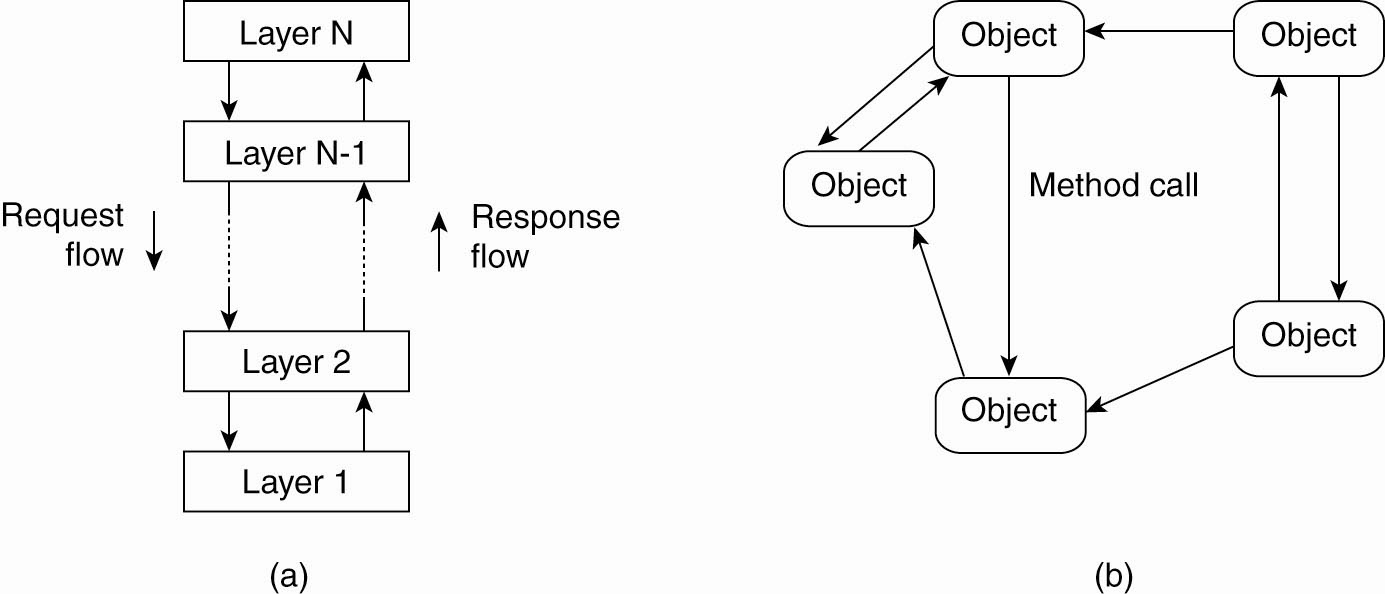
\includegraphics[width=0.5\textwidth]{images/layered}
      \caption{The layered (a) and object-based (b) architectural style}
      \label{layered}
    \end{figure}
  \item \textbf{Object based (figure~\ref{layered})}\\
    Here, objects can call other objects.
  \item \textbf{Event based (figure~\ref{event-based})}\\
    Often used as a publish-subscribe (pub-sub) architecture.
    \begin{figure}[H]
      \centering
      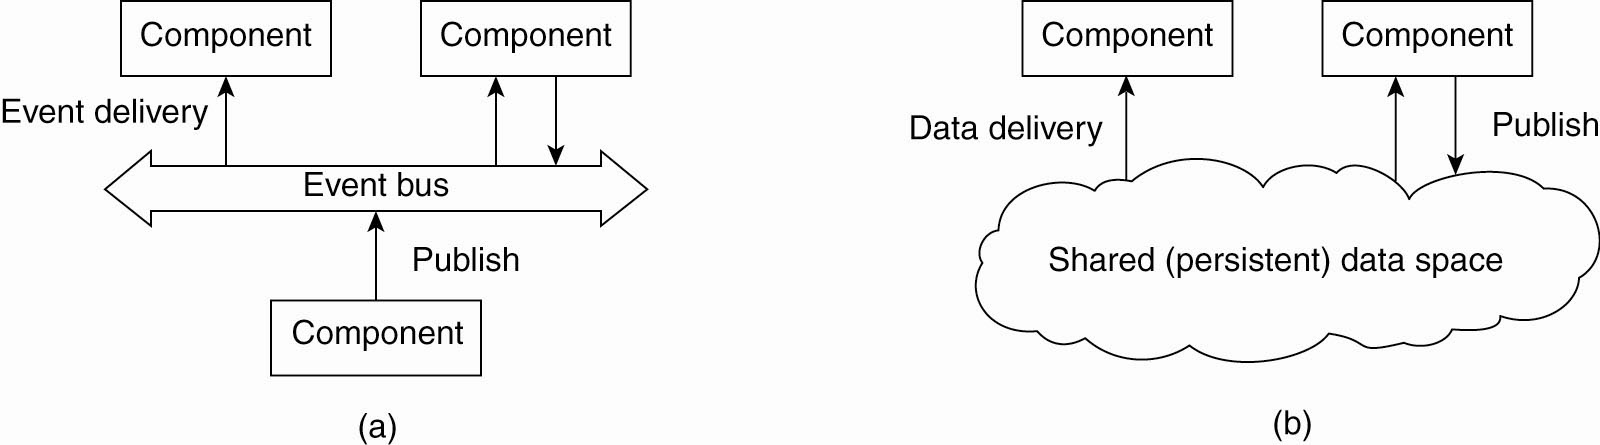
\includegraphics[width=0.5\textwidth]{images/event-based}
      \caption{The event-based (a) and shared-dataspace(b) architectural style}
      \label{event-based}
    \end{figure}
  \item \textbf{Shared dataspace (figure~\ref{event-based})}\\
    % TODO: Defo describe more
    \dots
\end{description}

\textbf{Middleware} is used to abstract away the complexity of dealing with
networks and their issues. Good middleware can effectively hide heterogeneity of
the underlying platforms (e.g. Windows x86 computers talking to Linux ARM
machines). The \textbf{end-to-end} argument reminds us of the limits of
middleware; and states that the functions specific to each application should
reside at the endpoints of the network, not the intermediary hosts. This means
that though middleware can provide generic functions for you to use, you still
have to apply these functions in your application in order to do something
useful.

\subsubsection{Client-Server model}

In this model, many clients will invoke functions on a remote server. Servers
(despite there being few of them) act as the slave, since they are passive and
wait for requests to come. Clients are masters, since they are active, and send
requests to servers. Servers can be stateful or stateless.

Client server architectures, by nature, are asymmetrical. As a result of this,
they often scale poorly, since the server load will increase proportional to the
number of clients. Of course, you can use multiple servers to spread the load on
any one server (horizontal scaling, done using proxies), and put caches between
the client and the server to server common and easy requests.

Another way to reduce the load on servers is to use `mobile code'. Popularised
by Java, this is when code is downloaded to a client from the server, and the
client executes the application locally. This reduces server load, and makes the
app responsive on the user's computer.

The opposite side to this, is having thin clients, who rely on the server to do
all of the heavy lifting for them (e.g. a very simple web browser like Lynx).

\subsubsection{Peer to Peer (P2P) model}

Here, all nodes in the network are the same, and they all talk to eachother.
These networks have no central point of coordination (or failure), which
provides resilience, yet at the same time, complexity.

Though P2P architectures scale well (since they are truly `distributed'), it is
hard to find, coordinate and use resources over the network because of a lack of
any central organisation.

% TODO: Checksums

\section{Remote Procedure Calls and Remote Method Invocation (RPC \& RMI)}

The basic idea of RPC and RMI is that a client will `call' a process on a remote
server to execute the code of a specific procedure, with a specific set of
arguments.

There are two ways that RPC calls are fulfilled; synchronous calls and
asynchronous calls. In a synchronous call, the idea is that the RPC call behaves
like a normal (local) procedure call, and the program running on the local
machine will stop executing until the RPC call has finished. In an asynchronous
call, the local program will carry on executing, until the remote method is
finished, at which point the remote machine will interrupt the local machine
telling it to process the results of the call.

\marginpar{Serialising parameters into transmittable and server-understandable
values is also called \textit{parameter marshalling}. Doing the opposite (when
the server receives the result) is called unmarshalling.}

Since the local and the remote clients are (or at least are designed to be)
running in different machines, the program arguments sent in the RPC call cannot
be references to addresses in memory; they must be serialised into values that
can be transmitted.

Some kind of middleware wrapper will handle the actual sending of messages over
the network. It will often provide `stub' methods to provide the service for
both the client and the server to make the system as transparent as possible.
This is shown in Figure~\ref{rpc-stub}

\begin{figure}[H]
  \centering
  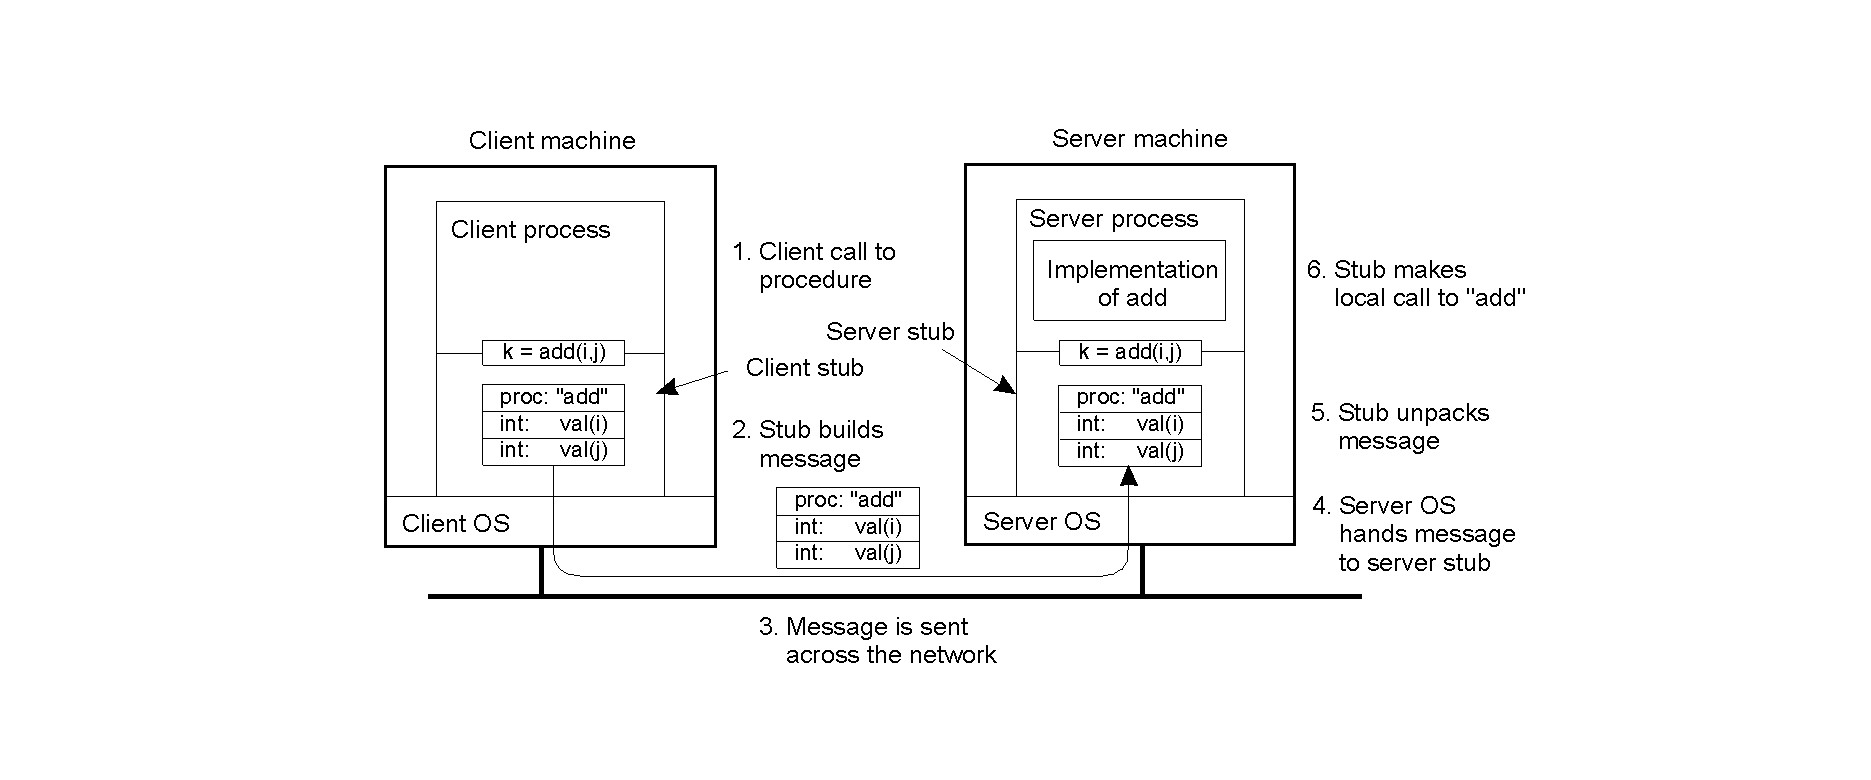
\includegraphics[width=\textwidth]{images/rpc-stub}
  \caption{How middleware stub methods could be used to facilitate RPC.}
  \label{rpc-stub}
\end{figure}

This middleware will have to be specific to the architecture \textit{it} is
running on, to make sure incoming data is passed to the program in the right
format (e.g. little-endian not big-endian). If we communicate using a language
and architecture independent medium such as a \textit{Interface Definition
Language}, then we can mostly avoid these pitfalls.

\subsection{Interface Definition Languages}

There are many different IDL's for example COBRA (Common Object Request Broker
Architecture) and DCE (Distributed Computing Environment).

A COBRA file might look like this:

\begin{lstlisting}
  // Person.idl
  struct Person {
    string name; 
    string place;
    long year;
  };
  interface PersonList {
    readonly attribute string listname;
    void addPerson(in Person p);
    void getPerson(in string name, 
        out Person p);
    long number();
  };
\end{lstlisting}

RMI is included in the standard Java API. To be able to send an \texttt{Object}
as a parameter, it must implement \texttt{Serializable}, which is an interface
that lets you turn the object into a byte stream and back again. Having
\texttt{Serializable} objects is good because it allows you to create
arbitrarily nested serializable objects.

A major difference between RMI and RPC is that RMI can reference remote objects.
The stub based architecture is similar, except the stub will forward the message
to a per-class \texttt{dispatcher}, which then sends the message to the
receiver's \texttt{skeleton} that handles unmarshalling. The \texttt{skeleton}
will reply with another message to the dispatcher when the request finishes
containing the result or any exceptions.

Remote objects are made available to RMI clients by exposing the
\texttt{rmiregistry} which is a key-object store on the server. Clients
interrogate the registry using the String that corresponds to the object they
want.

\subsubsection{Parameter passing}

It is important to note that programming languages can use two different methods
of passing parameters between functions; call by reference and call by value.
The former is where you pass the function a pointer to a memory location (where
a thing (object, value etc) is stored), while in the latter you actually pass
the object/value directly to the function. If you're using RPC, then you need to
use call by value, since the pointer you would pass with call by reference is
meaningless to the remote machine.

This means you will have to \textit{serialise} any parameters that you want to
send along with an RPC call. To serialise and deserialise an object, you need to
be able to convert it into text (it can be human readable, such as JSON, or just
binary data in ascii format) and back again.

\subsection{Connecting and binding to an RPC server}

Obviously, it would be silly to hard code the details of the server into client
applications. Instead we can use a directory server (at a known location) to
tell us the IP address and port of the server we want. The server can use a
process to allocate different ports to different connections.

\begin{figure}[H]
  \centering
  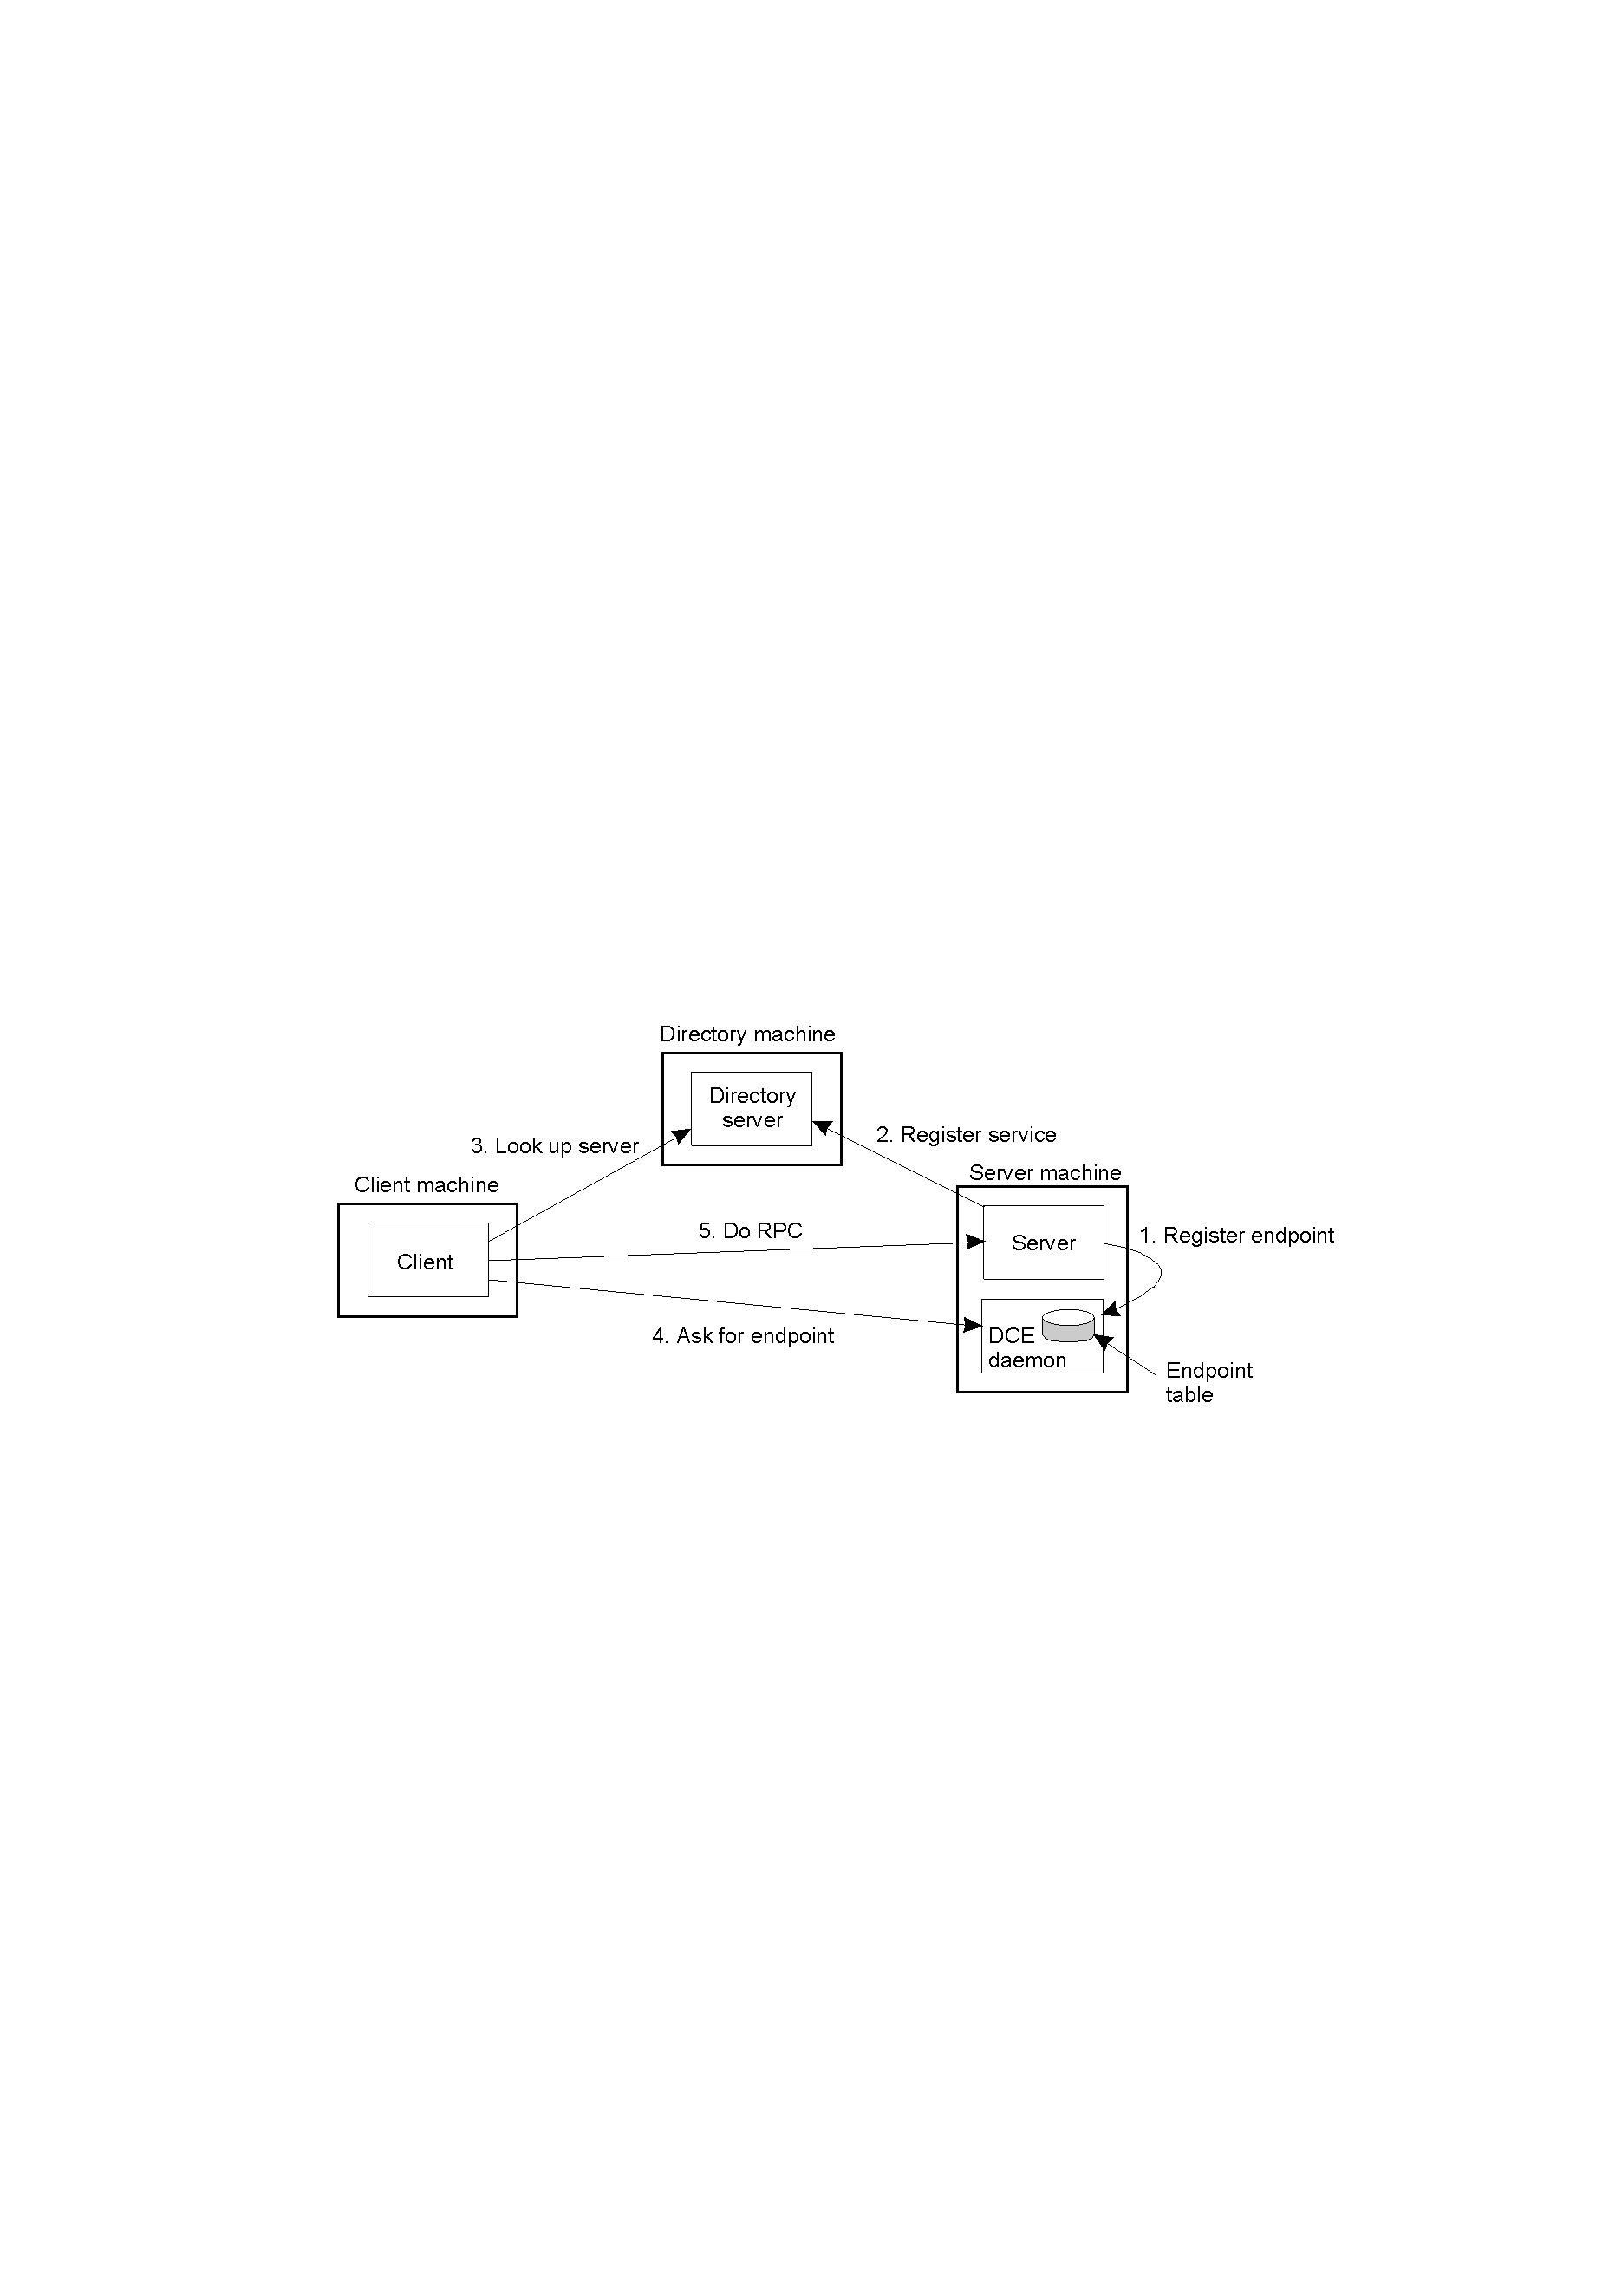
\includegraphics[width=\textwidth]{images/directory-server}
  \caption{How a directory server can be used can be used to find the location
  and port of the remote server.}
  \label{rpc-stub}
\end{figure}

\subsubsection{Name resolution}

Names can be \textit{pure} or \textit{non-pure}. Pure names contain no
information about the item they are associated with, while non-pure names do. An
address is a non-pure name, since it tells you exactly where to find a server.

When a name is \textit{resolved}, it is translated into data about the item it
describes. Names are bound to attributes such as addresses, and as such, can
often be directly used in resolution. For example, in a URL, you have the
format:

\begin{verbatim}
  http://{domain name}:{port}/{path}
\end{verbatim}

The domain name (such as example.com) can be resolved into an IP address using a
DNS lookup. This can be used in conjunction with the port and path to accurately
describe where a resource is on the internet.

There are three different, yet commonly used names for the web:

\begin{description}
  \item \textbf{U}niform \textbf{R}esource \textbf{I}dentifiers\\
    These identify resources on the web, and start with a URI scheme such as
    \texttt{http:}, \texttt{ftp:}, \texttt{ssh:} etc.
  \item \textbf{U}niform \textbf{R}esource \textbf{L}ocators\\
    These are a subset of URI's that give a location for a resource.
  \item \textbf{U}niform \textbf{R}esource \textbf{N}ames\\
    An URI which is not a URL. All URN's begin with \texttt{urn:}.
\end{description}

Names can also be flat, or hierarchical. If the name is flat, then it can be
resolved all at once, but if it is hierarchical, then you have to resolve each
part of the name in a different context.

Obviously, DNS is the most well known name resolution mechanism; it is
responsible for turning URLs into IP addresses. Replication and caching are used
to make the system able to handle the load. Since the data is very large, it is
partitioned by the domain.

Name resolution can be implemented recursively (Figure~\ref{recursive-
resolution}), or iteratively (Figure~\ref{iterative-resolution}). In the former
case, the whole name is sent to the root nameserver which resolves the top most
part, and forwards it on to the next nameserver, which continues until the name
has been fully resolved, at which point, it is sent back to the client. An
iterative method would have the client poll each different nameserver in turn
for a resolution of part of the name.

\begin{figure}[H]
  \centering
  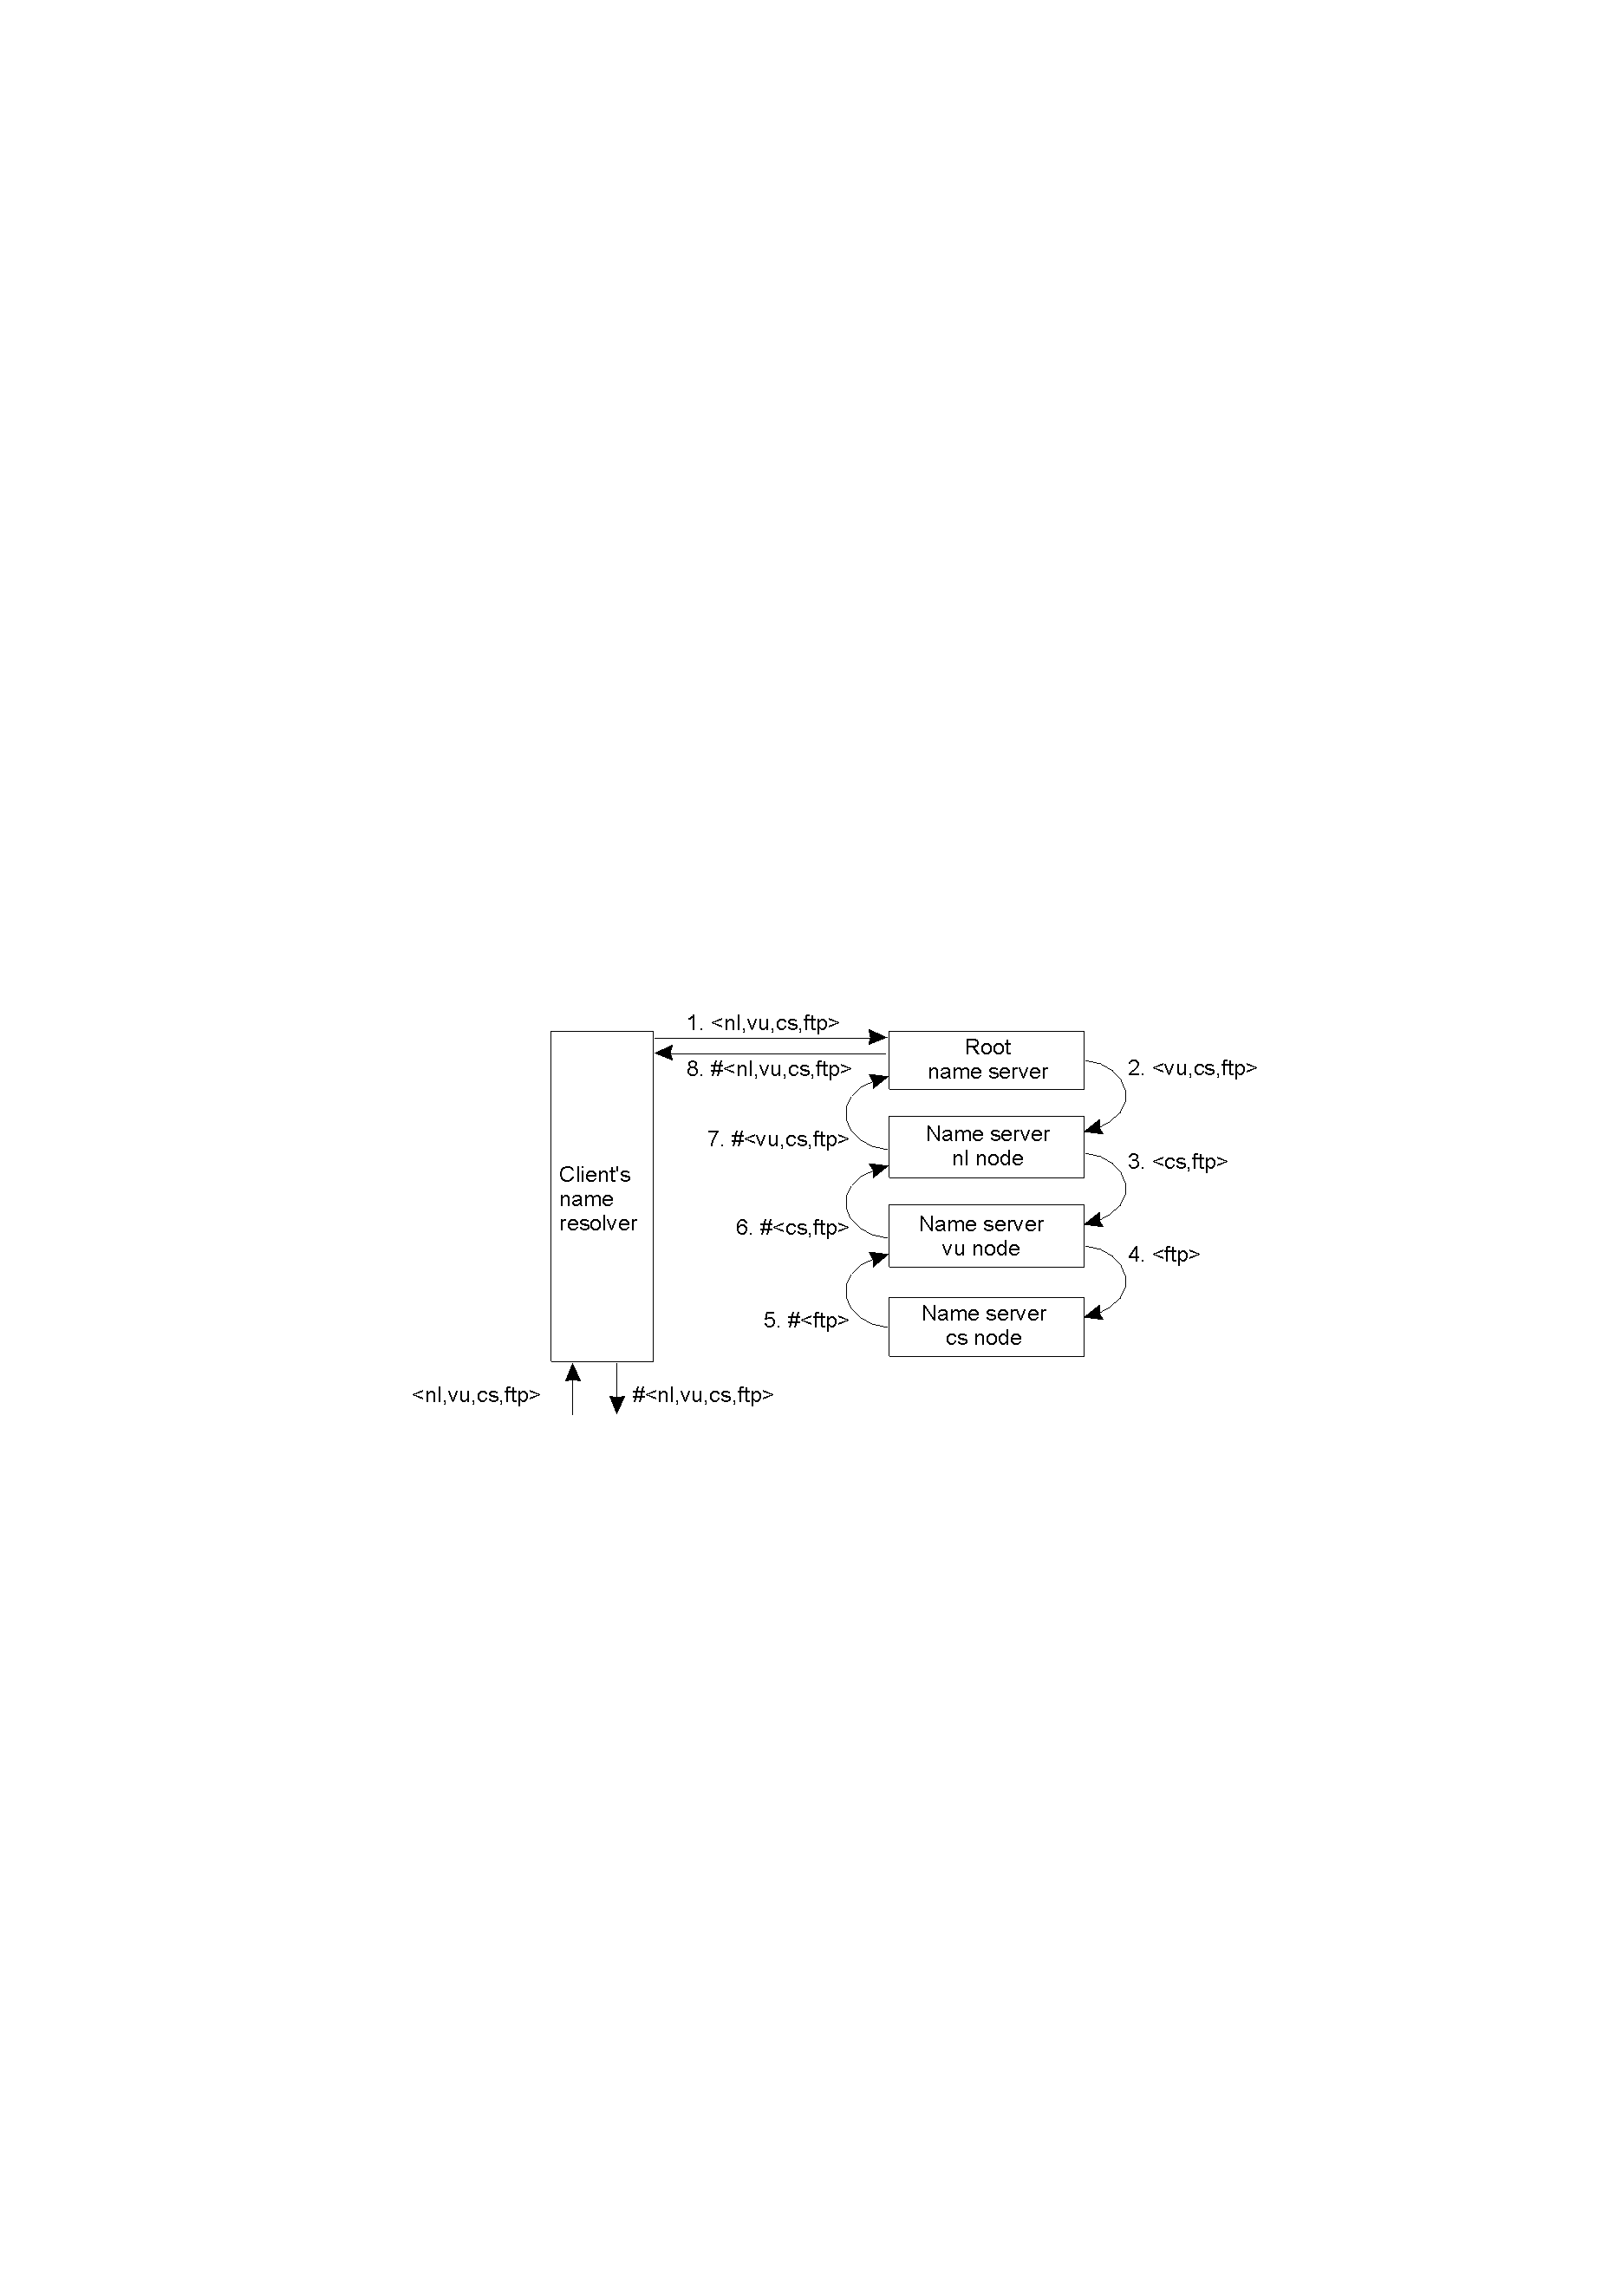
\includegraphics[width=\textwidth]{images/recursive-resolution}
  \caption{Recursive domain name resolution.}
  \label{recursive-resolution}
\end{figure}

\begin{figure}[H]
  \centering
  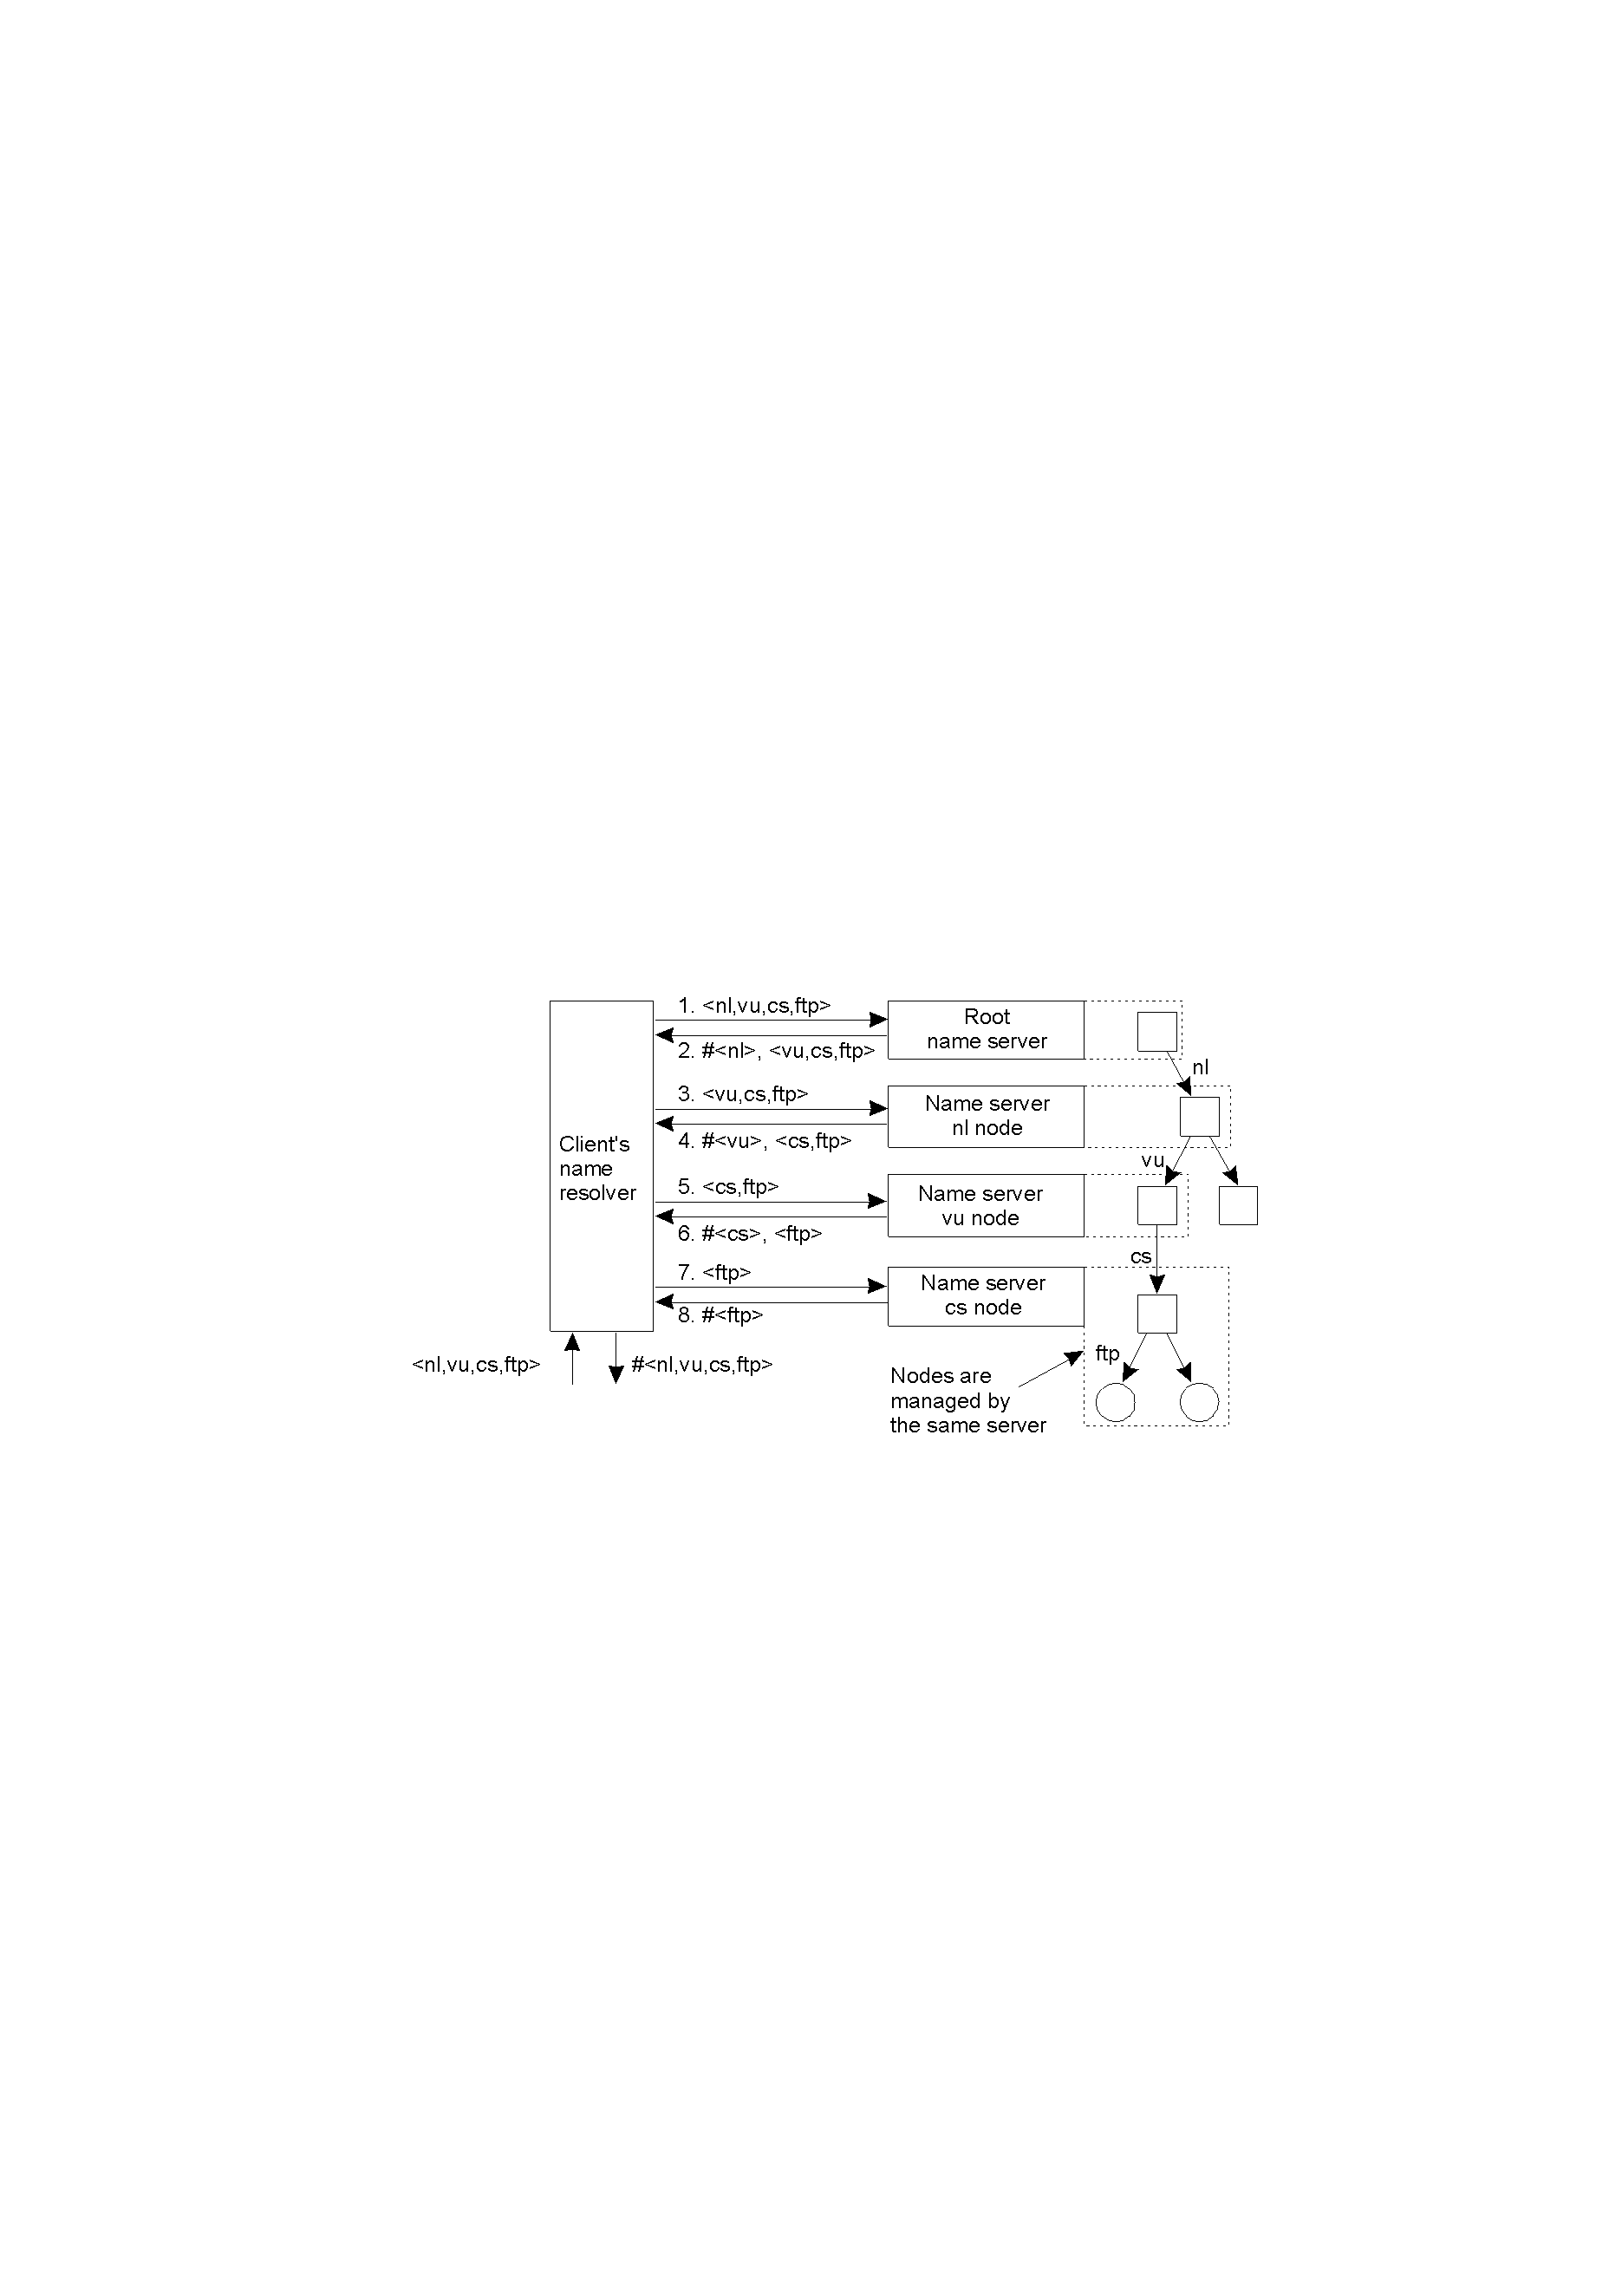
\includegraphics[width=\textwidth]{images/iterative-resolution}
  \caption{Iterative domain name resolution.}
  \label{iterative-resolution}
\end{figure}

Recursive resolution puts more burden on the name server, but also makes it
easier to program clients, and also can improve caching (since the caches are
centralised at the nameserver).

\section{LDAP}

The Lightweight Directory Access Protocol is a way of querying for information
about services. LDAP works on top of the Internet Protocol, and provides a
distributed directory information service.

%TODO: Either move this somewhere else or add much more information ;)

\section{Time and clocks}

Being able to agree on a single clock is very advantageous in distributed
systems, however, setting distributed systems to be set to the same time, and
keeping them in time once they are is an issue.

\subsection{UTC}

Coordinated Universal Time is a time standard commonly used around the world.
International Atomic Time is kept by around 200 atomic oscillators around the
world, each with a drift rate of around 1 in $10^13$ seconds. Astronomical time
is derived from stars and the sun, but diverges slightly because the earth's
rotation is slowing. UTC is based off atomic time, but leap seconds are
occasionally inserted so that it is in time with astronomical time. UTC is
broadcast by satellites and radios.

GPS receivers are accurate to about one millisecond, whilst receivers from
radios or telephone lines are accurate to a few milliseconds. Inexpensive
crystal clocks have a drift of around 1 in $10^6$ seconds, and this is usually
what computers are accurate to.

\subsection{Setting times}

There are multiple ways of reaching a consensus about times between different
machines:

\begin{description}
  \item \textbf{Cristian's method}:\\
    Here, a time server is polled by clients and returns the time on the server.
    The client times how long it took for the round trip time, divides it by two
    and adds it to the time that the server returned. This works well for short
    round trip times.
  \item \textbf{Berkeley Algorithm}:\\
    The Berkeley algorithm has one master that polls other slaves. Each slave 
    replies with its own time, and the master estimates their local times (using
    Cristian's method). The master then averages all of the slaves times and its
    own time, and eliminates any times with an excessive round trip time and any
    obvious outliers.

    Once the master has determined the time, it then sends each clock a delta, 
    which is how much to add or take off its own clock. If the master fails, 
    then a distributed election algorithm elects a slave as the replacement.
  \item \textbf{Network Time Protocol (NTP)}:\\
    NTP is designed for large scale internet (as opposed to the other two, which
    were designed for smaller scale networks). There is a network of servers,
    one is primary and the others are secondary. The primary server will have
    a UTC clock.

    There are three methods of synchronisation; multicast mode, procedure call
    mode and symmetric mode.

    \begin{description}
      \item \textit{Multicast mode}:\\
        Multicast mode is used on high speed LAN's and is not accurate. The time
        is broadcast to clients from the server at intervals, and the clients
        set their time equal to the received time plus a little bit for latency.

      \item \textit{Procedure call mode}:\\
        This mode is very similar to Cristian's algorithm. The server basically
        just accepts requests and replies with the time. This is more accurate
        than multicast mode, and is used when accuracy is key, or multicast is 
        not supported.

      \item \textit{Symmetric mode}:\\
        This is the most accurate of the three; messages are exchanged and data
        is build up to improve the accuracy of the time as more messages are 
        send and received. Each message contains time information about the
        previous message.

        Each NTP server will interact with several peers to identify which ones
        are the most reliable. This can achieve accuracies of from
        $10-100\si{\milli\second}$ over the Internet.
    \end{description}
\end{description}

\subsection{Logical time}

In a single processor, every event can be ordered in time using the local clock.
However, if we are in a distributed system, then the synchronization between
clocks may not be good enough to do this.

If any two events happen in a process, they occur in the order given by the
process. If a message is sent from one process to another, then the act of
sending and that of receiving is said to be an event. This defines a partial
ordering of events, given by the \textit{happens-before} relationship.

A logical clock is a monotonically (i.e. increases by one) increasing counter.
Each process keeps its own logical clock and uses it to timestamp its own
events. When a message is received, then the clock is updated to be the logical
time of the received message, or the current logical time (whichever is
highest), plus one.

A \textbf{Vector Clock} is similar to the \textbf{Lamport Clock} described
above, but each process keeps track of the clock of each other process. It is in
essence $n$ Lamport clocks, one for each process. When a process receives a
message, it \textit{merges} its clock with the clock in the message, fining the
max of each item.

Vector clocks capture causality which Lamport clocks do not, however, vector
clocks are more expensive in terms of bandwidth.

\section{Elections, coordination and agreement}

Implementing a semaphore is a common task for computer scientists.
\marginpar{See my COMP25111 notes for stuff on semaphores.} On a single machine,
even on one with multiple processors, this is fairly easy to implement, but when
memory isn't shared (like in a distributed system), then we can't just have a
semaphore in memory; we need some system to manage access.

The simplest of these systems is a central server, where a client requests a
token on entry of a critical section, and releases it on exit. Processes are
held in a queue until there is a free slot for them to enter their critical
section.

The trouble with this though, is that the server is a single point of failure,
and if the critical sections are short or the server is slow etc, then the
server could become a bottleneck.

\subsection{Elections}

If the server `goes down', then no processes would be able to enter their
critical sections. Obviously this is \textit{slightly} detrimental to the
running of the system, so ideally we would like a way of replacing the server if
crashes.

If we have $n$ clients/processes, and we want to select one to be a server, then
it makes sense to select one that has the lowest load. We could give each server
an identifier, which is a pair of $\frac{1}{load + 1}$ and $i$, where $i$ is the
number (or unique ID) of the client.

We also need to make sure that all the clients can learn about and agree on the
result of the election, and let any client initiate an election at any time (so
we could have multiple elections concurrently occurring).

\subsubsection{Ring-based election algorithm}

If we arranged the processes in a logical ring, then each process knows which is
next in the order (this assumes there are no failures in the system).

\begin{enumerate}
  \item Initially, all processes are non-participants in the election.

  \item The initiating process changes itself to be a participant and sends its
  identifier (remember, that's $\frac{1}{load + 1}$) to its neighbour).

  \item Each receiver will forward its own identifier if it is higher than the
  one it received. If it is already a participant (i.e. its forwarded an
  identifier previously), then the message is discarded. If the received
  identifier is lower than its own identifier, the node forwards its own 
  identifier.

  \item If the identifier of the receiving process is the same as the received 
  identifier, then that process has been elected. It now sends an elected
  message around informing the other nodes of its ascension to serverhood.

  \item When each node receives an election result, it reset to
  non-participating and passes the result on.
\end{enumerate}

The largest number of messages sent is $3n -1$ which isn't too bad. However,
failure tolerance is limited (you could re-build the ring if one node crashed,
but that's a lot of effort) and its hard to add new clients to the ring.

\subsubsection{Bully algorithm}

The bully algorithm is designed to be more resilient, since it takes into
account that processes may crash (although messages are still assumed to be
reliable). Each process knows about each other process and they can all
communicate with each other.

Timeouts are used to detect the failure of processes. If a reply has not been
received in a time $T$, then the replying process is assumed to have crashed. If
the initiator of an election doesn't learn who has won by $T^1 + T^2$, then it
assumes some process crashed and it starts another election.

Three types of messages are used to communicate:

\begin{description}
  \item \textbf{Election messages} are sent to initiate an election
  \item \textbf{Answer messages} are sent in response to election messages
  \item \textbf{Coordinator messages} are sent to announce election winners
\end{description}

This is how the method works:

\begin{enumerate}
  \item The initiating client will send a message to all the clients with a
  higher identifier than itself. The initiator now waits for the result.

  \item Any client that receives an election message eventually will send an
  answer back. It should then start its own election, by sending a message to
  clients that have a higher identifier than it.

  \item Only when a process gets no replies (within the timeout), does it
  consider itself elected, at which point, it sends a coordinator message to all
  lower processes.
\end{enumerate}

This process if $O(n^2)$ in the worst case, which is where the smallest process
initiates. Timeouts must be realistic, otherwise the election can be slow.
